\documentclass{article}
\usepackage{amsmath,mathtools}
\usepackage[utf8]{inputenc}
\usepackage[ngerman]{babel}
\usepackage{acronym}
\usepackage{graphicx} 
\usepackage{epstopdf}
\usepackage{svg}
\usepackage{multirow}

%Hyperlinks package, links aus inhaltsverzeichnis
\usepackage{hyperref}
\hypersetup{
    colorlinks=false, %set true if you want colored links
    linktoc=all
}
%Blattformatierung
\usepackage{geometry}
\geometry{a4paper, top=25mm, left=30mm, right=25mm, bottom=20mm}


\def\presuper#1#2%
	{\mathop{}%
	\mathopen{\vphantom{#2}}^{#1}%
	\kern-\scriptspace%
	#2}
%Display vecotr in a reference frame
\newcommand{\vecBS}[4]{\presuper{#1}{\begin{pmatrix}
#2 \\ #3 \\ #4
\end{pmatrix}}}
%Boldsymbol shortcut
\newcommand{\bs}[1]{\boldsymbol{#1}}
%Bezugssystemdefinition
\newcommand{\defBS}[1]{\{#1\} [ \bs{e}_{{#1}_1},\bs{e}_{{#1}_2}, \bs{e}_{{#1}_3} ]}
%Projektionsmatrix
\newcommand{\pMat}[2]{\presuper{#1}{\bs{P}}^{#2}}
%Differenation in Respekt zu BS
\newcommand{\diffIn}[3]{\frac{\presuper{#1}{d{#2}}}{d#3}}
\newcommand{\partialDiffIn}[3]{\frac{\presuper{#1}{\partial{#2}}}{\partial #3}}
%Geschwindigkeit/Beschleunigung
\newcommand{\vel}[3]{\presuper{#1}{\bs{#2}}^{#3}}

%Rightarrow with spaceing
\newcommand{\rArrow}{\hspace{5pt}\rightarrow\hspace{5pt}}
%Inneres Produkt
\newcommand{\inProd}[2]{\langle {#1}, {#2} \rangle}

%System macro
\newcommand{\cSS}[3]{\textfrak{S}($\bs{#1}$,$\bs{#2}$,$\bs{#3}$)}
\newcommand{\dSS}[3]{\textfrak{D}($\bs{#1}$,$\bs{#2}$,$\bs{#3}$)}

%Laplace transform sign with spaces
\newcommand{\myLaplace}{\hspace{15pt}\laplace\hspace{15pt}}

\newcommand*{\signed}[1]{%
        \nolinebreak[3]\hspace*{\fill}\mbox{\emph{#1}}
    }

\begin{document}
\tableofcontents
\section{Modellbildung Würfelseite}
Die Untersuchung des Systems beginnt mit der Bestimmung eines mathematischen Modells, welches in diesem Abschnitt näher erläutert wird.  Zunächst beschränkt sich die mechanische Untersuchung auf einen vereinfachten Prototypen, welcher aus einer Würfelseite besteht, die auf einer Achse gelagert ist. An der Würfelseite ist ein Motor befestigt, auf dessen Schaft wiederum eine Schwungmasse gelagert ist. Die Herleitung der Bewegungsgleichungen erfolgt mit Hilfe der Methoden nach Kane [Kane], die im Verlauf der Untersuchung näher erläutert werden

\subsection{Untersuchung der Kinematik}
Zu Beginn der Untersuchung werden die kinematischen Zusammenhänge mit Hilfe von Bezugssystemen beschrieben. Dieser Ansatz ist bereits aus der Relativkinematik bekannt, wobei häufig nur zwischen einem Inertial- und Relativsystem unterschieden wird. Allerdings kann diese Prinzip auf eine beliebige Anzahl von Bezugssystemen erweitert werden.

\begin{figure}[!h]
\centering
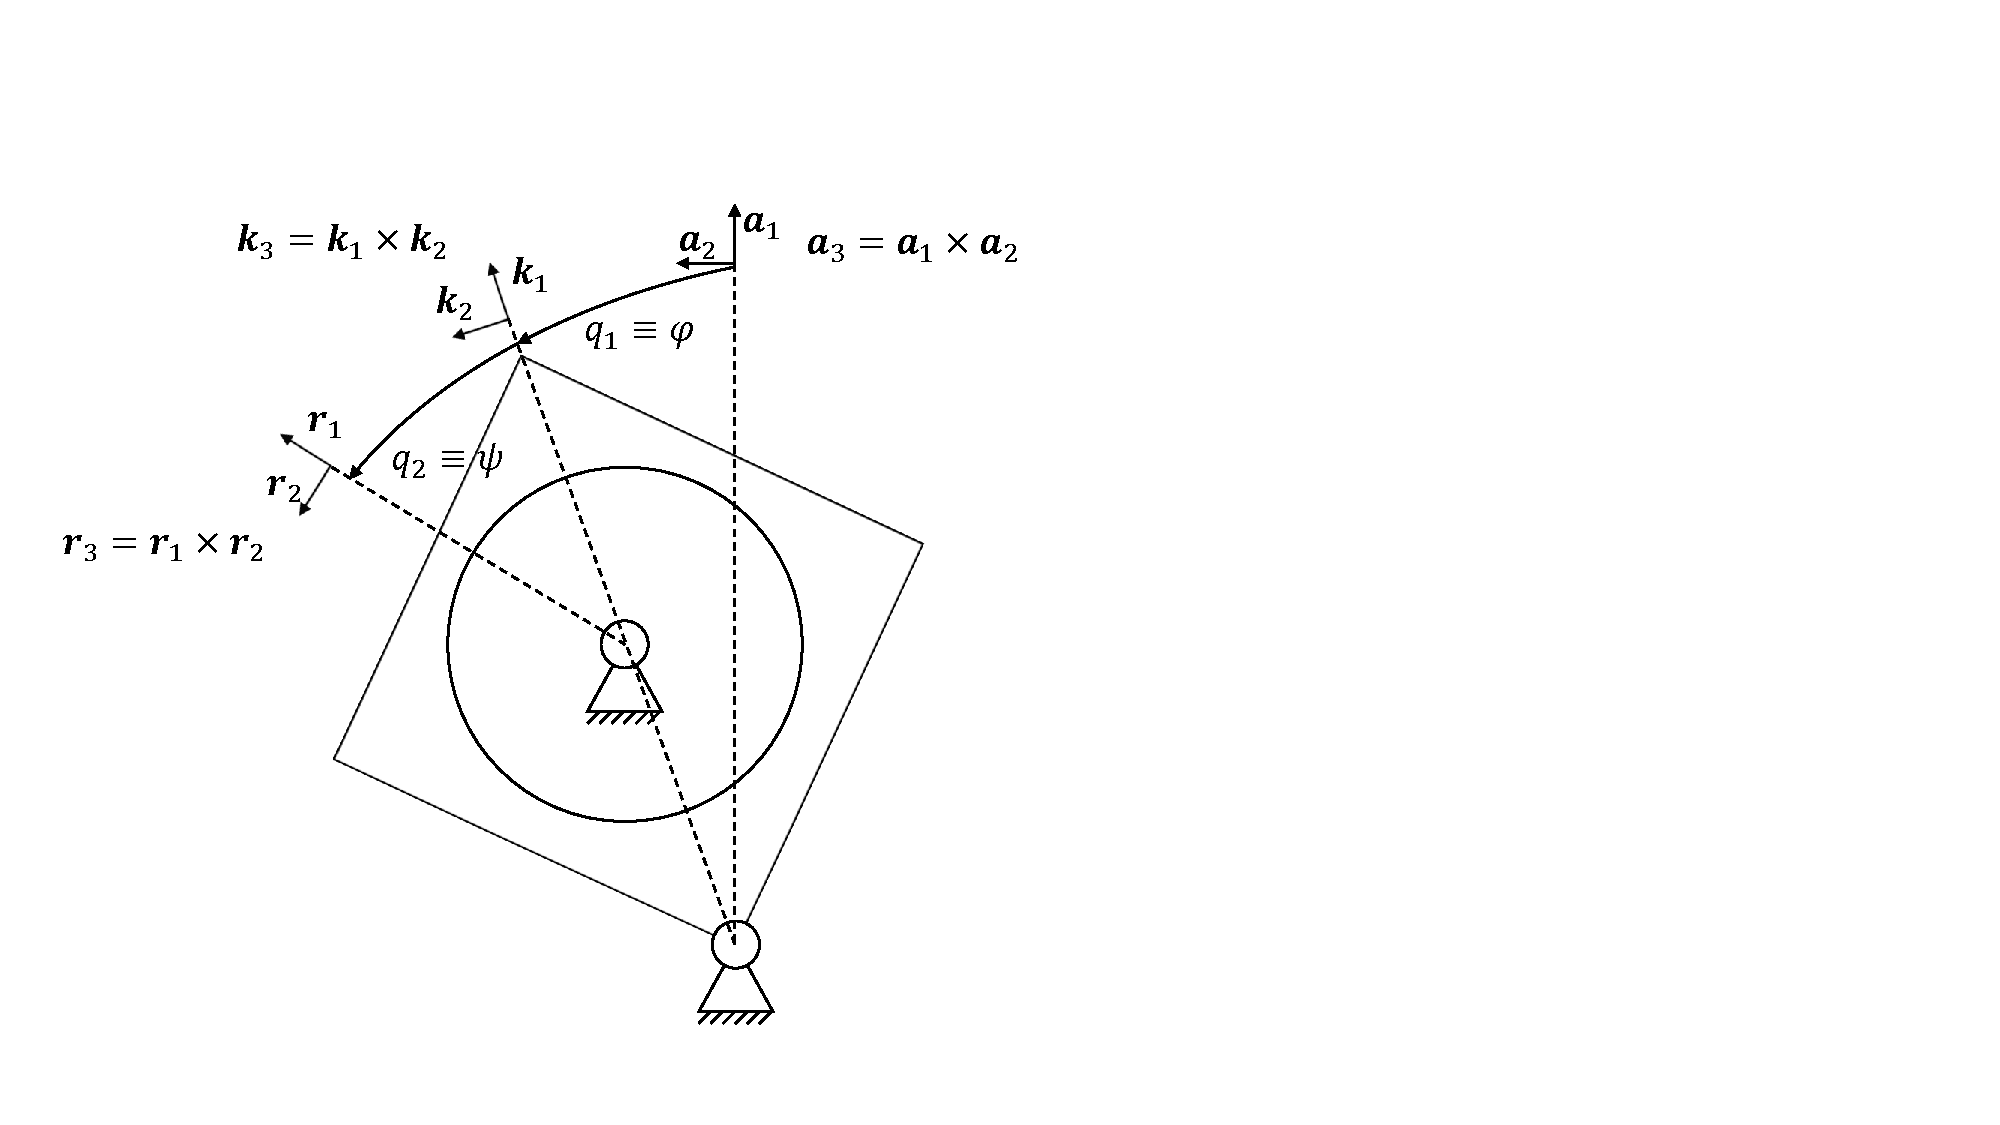
\includegraphics[width=0.6\linewidth, trim={1cm 1.5cm 18cm 3.5cm}, clip]{2_ModellWuerfelseite/img/ModellWuerfelseite}
\caption{Mechanischer Aufbau der Würfelseite, Quelle: eigene Darstellung}
\label{abb_wuerfelseite}
\end{figure}

Ein Bezugssystem $A$ wird durch drei Vektoren $\bs{a}_i \hspace{5pt} i \in {1, 2, 3}$ definiert, welche auch als Vektorbasis des Bezugssystem bezeichnet werden. Prinzipiell müssen diese drei Vektoren nur linear unabhängig sein, allerdings werden in dieser Arbeit ausschließlich paarweise orthogonale Einheitsvektoren verwendet, da diese eine leichtere Handhabung ermöglichen. Ist ein Bezugssystem definiert kann ein beliebiger Vektor $\bs{v}$ als Linearkombination der Vektorbasis ausgedrückt werden. Als Beispiel sei hierfür das Bezugssystem $K$ genannt, welches durch die die Einheitsvektoren $\bs{k}_i$ definiert ist. Diese sind nach \ref{abb_wuerfelseite} an der Würfelseite fixiert, d.h. die Ausrichtung der Einheitsvektoren ändert sich mit der Rotation der Würfelseite. 
\begin{equation}
\bs{v} = v_{k1} \bs{k}_1 + v_{k2} \bs{k}_2 + v_{k3} \bs{k}_3 = \vecBS{K}{v_1}{v_2}{v_3}
\end{equation}
Da im Verlauf der Untersuchung mehrere Bezugssysteme eingeführt werden, muss die vektorielle Schreibweise neben den einzelnen Komponenten auch das verwendete Bezugssystem wiedergeben. Dies erfolgt durch den vorangehenden Superskript. 
Um die Bedeutung der Vektorbasis zu veranschaulichen wird im nächsten schritt das Intertialsystem $A$ mit der Vektorbasis $\bs{a}$ definiert. Da es sich bei $A$ um ein Intertialsystem handelt ändert sich die Ausrichtung der Vektoren $\bs{a}_i$ im Verlauf der Zeit nicht. Solche Systeme werden auch als im Raum fixierte bzw. raumfeste Bezugssysteme bezeichnet. Nun kann der Vektor $\bs{v}$ auch als Linearkombination der Vektoren $\bs{a}_i$ dargestellt werden. Man nennt diese  Form des Vektors auch dessen Darstellung aus Perspektive von $A$.
\begin{equation}
\bs{v} =  v_{a1} \bs{a}_1 + v_{a2} \bs{a}_2 + v_{a3} \bs{a}_3 = \vecBS{A}{v_{a1}}{v_{a2}}{v_{a3}}
\end{equation}
Nun stellt sich die Frage wie die beiden Darstellungen des Vektors $\bs{v}$ zusammenhängen. Die Komponente eines Vektors $\bs{v}$ in Richtung eines Einheitvektors $\bs{k}_i$ ergibt sich aus deren Skalarprodukt ([Kane], S. 23ff). Wird dieser Ansatz auf alle drei Komponenten appliziert ergibt sich am Beispiel der beiden Bezugssysteme $A$ und $K$ die folgende Gleichung.
\begin{equation}
\begin{split}
\bs{v} &= \inProd{\bs{v}}{\bs{k}_1} \bs{k}_1 + \inProd{\bs{v}}{\bs{k}_2}\bs{k}_2 + \inProd{\bs{v}}{\bs{k}_3}\bs{k}_3 = \vecBS{K}{\inProd{\bs{v}}{\bs{k}_1}}{\inProd{\bs{v}}{\bs{k}_2}}{\inProd{\bs{v}}{\bs{k}_3}} \\
&= \vecBS{K}{v_{a1}\inProd{\bs{a}_1}{\bs{k}_1} + v_{a2}\inProd{\bs{a}_2}{\bs{k}_1} + v_{a3}\inProd{\bs{a}_3}{\bs{k}_1}}{v_{a1}\inProd{\bs{a}_1}{\bs{k}_2} + v_{a2}\inProd{\bs{a}_2}{\bs{k}_2} + v_{a3}\inProd{\bs{a}_3}{\bs{k}_2}}{v_{a1}\inProd{\bs{a}_1}{\bs{k}_3} + v_{a2}\inProd{\bs{a}_2}{\bs{k}_3} + v_{a3}\inProd{\bs{a}_3}{\bs{k}_3}}
= \presuper{K}{\begin{pmatrix}
\underbrace{
\begin{bmatrix}
\inProd{\bs{a}_1}{\bs{k}_1} & \inProd{\bs{a}_2}{\bs{k}_1} & \inProd{\bs{a}_3}{\bs{k}_1} \\
\inProd{\bs{a}_1}{\bs{k}_2} & \inProd{\bs{a}_2}{\bs{k}_2} & \inProd{\bs{a}_3}{\bs{k}_2} \\
\inProd{\bs{a}_1}{\bs{k}_3} & \inProd{\bs{a}_2}{\bs{k}_3} & \inProd{\bs{a}_3}{\bs{k}_3}
\end{bmatrix}}_{\equiv \pMat{A}{B}} \cdot \underbrace{\begin{bmatrix}
v_{a1} \\ v_{a2} \\ v_{a3}
\end{bmatrix}}_{= \presuper{K}{\bs{v}}}
\end{pmatrix}} 
\\
&= \presuper{K}{\begin{pmatrix}
\begin{bmatrix}c_{\varphi} & s_{\varphi} & 0 \\ -s_{\varphi} & c_{\varphi} & 0 \\ 0 & 0 & 1 \end{bmatrix} \cdot \presuper{K}{\bs{v}} \end{pmatrix}}
\end{split}
\end{equation}
Folglich kann der Zusammenhang zwischen den Darstellung von $\bs{v}$ aus den Perspektiven von $A$ und $K$ als lineare Abbildung ausgedrückt werden, welche durch die Matrix $\pMat{A}{K}$  definiert ist. Diese Matrix hängt von dem Winkel $\varphi$ ab, welcher eine generalisierte Koordinate ist und einen rotatorischen Freiheitsgrad des Systems beschreibt. Der zweite Freiheitsgrad des Systems ensteht durch die Rotation der Schwungmasse relativ zu der Würfelseite. Diese Drehung wird von dem Winkel $\psi$ beschrieben. Wird nun ein weiteres Bezugssystem $R$ eingeführt, dessen Vektorbasis $\bs{r}$ auf der Schwungmasse fixiert ist kann der Zusammenhang der Bezugssysteme $K$ und $R$ wieder mit einer Abbildungsmatrix $\pMat{K}{R}$ beschrieben werden.
\begin{equation}
\pMat{K}{R} = \begin{pmatrix}
c_{\psi} & -s_{\psi} & 0 \\ s_{\psi} & c_{\psi} & 0 \\ 0 & 0 & 1
\end{pmatrix}
\end{equation}
Die Vorteile dieser Beschreibungsform zeigen sich, wenn man zum Beispiel das Moment $\bs{T}^{G/O}$ berechnen möchte, welche durch die Gravitationskraft $\bs{G}$ verursacht wird. Dieser Kraftvektor lässt sich leicht aus der Perspektive des Intertialsystems $A$ bestimmen.
\begin{equation}
\bs{G} = \vecBS{A}{-g\cdot m}{0}{0}
\end{equation}
Des weiter hängt das Gravitationsmoment von dem Ortsvektor $\bs{c}$ des Schwerpunktes $C$ ab, der mit Hilfe einer CAD-Anwendung aus der Perspektive von $K$ ermittelt wird.
\begin{equation}
\bs{c} = \vecBS{K}{l_C}{0}{0}
\end{equation}
Um nun das Gravitationsmoment zu berechnen muss das Kreuzprodukt der beiden Vektoren gebildet werden. Hierfür müssen die Vektoren aber aus Perspektive des selben Bezugssystems dargestellt werden. Dies erfolgt mit Hilfe der Abbildungsmatrix $\pMat{K}{A}$.
\begin{equation}
\begin{split}
\bs{T}^{G/O} &= \bs{c} \times \bs{G} = \presuper{A}{\begin{pmatrix}
\pMat{K}{A} \cdot \vecBS{K}{l_C}{0}{0}
\end{pmatrix} \times \vecBS{A}{-g\cdot m}{0}{0}} \\
&= \vecBS{A}{c_{\varphi}\cdot l_C}{s_{\varphi}\cdot l_C}{0} \times \vecBS{K}{-g\cdot m}{0}{0} = \vecBS{A}{0}{0}{m\cdot g\cdot l_C \cdot s_{\varphi}}
\end{split}
\end{equation}
Dieses Beispiel zeigt, dass die Einführung von Bezugssystemen eine eindeutige Notation und Vorgehensweise zur Berechnung von Vektoren ermöglicht. Man möge bei diesem Anwendungsfall zwar argumentieren, dass die trigonometrischen Zusammenhänge des Gravitationsmoment auch direkt aus Abbildung \ref{abb_wuerfelseite} gewonnen werden können und keine Abbildungsmatrizen notwendig sind. Allerdings zeigt die Untersuchung des Würfels, dass die obige Vorgehensweise auf Beispiele beliebiger Komplexität angewandt werden kann. 

Des weiteren stellt der Ortsvektor $\bs{c}$ des Schwerpunktes ein gutes Beispiel dar um die Ableitung eines Vektors zu diskutieren. Aus Perspektive des Bezugssystem $K$ ist der Vektor $\bs{c}$ konstant. Wird der Vektor aber in $A$ abgebildet so hängt dieser von der Zeitfunktion $\varphi(t)$ ab. Deshalb muss bei der Ableitung eines Vektors das Bezugssystem angegeben werden, aus dessen Perspektive die Differentation durchgeführt werden soll ([Kane], S. 25 ff.). Wenn beispielsweise der Vektor $\bs{c}$ in $A$ differenziert werden soll, so muss dieser zunächst in $A$ dargestellt werden und anschließend seine Komponenten nach der Zeit abgeleitet werden. 
\begin{equation}
\frac{\presuper{A}{d \bs{c}}}{dt} = \frac{d(c_{\varphi}\cdot l_C)}{dt}\bs{a}_1 + \frac{\presuper{A}{d(s_{\varphi}\cdot l_C})}{dt}\bs{a}_2 + \frac{\presuper{A}{d (0)}}{dt}\bs{a}_3 = \vecBS{A}{-s_{\varphi}\cdot \dot{\varphi}\cdot l_C}{c_{\varphi}\cdot \dot{\varphi}\cdot l_C}{0}
\end{equation}
Aus dieser Überlegung resultiert auch die Frage wie sinnvoll die, aus der klassischen Mechanik bekannte, Definition der Geschwindigkeit als Ableitung des Ortes nach der Zeit ist, da diese keinerlei Abhängigkeit eines Bezugssystemes beinhaltet. Deshalb führt Kane anstelle der Geschwindigkeit $\bs{v}$ eines Punktes $P$, die  Geschwindigkeit $\vel{A}{v}{P}$ bzw. Beschleunigung $\vel{A}{a}{P}$ eines Punktes relativ zu dem Bezugssystem $A$ mit der folgenden Definition ein ([Kane], S. 28).
\begin{equation}
\vel{A}{v}{P} = \frac{\presuper{A}{d\bs{p}}}{dt} \hspace{35pt} \vel{A}{a}{P} = \frac{\presuper{A}{d\vel{A}{v}{P}}}{dt}
\end{equation}
Die selbe Notation wird für Winkelgeschwindigkeiten und -beschleunigungen eingeführt, wobei $\vel{A}{\omega}{B}$ die Winkelgeschwindigkeit bzw. $\vel{A}{\alpha}{B}$ die Winkelbeschleunigung des Punktes oder Bezugssystems $B$ relativ zu $A$ ist. Die Geschwindigkeit relativ zu einem Intertialsystem wird auch als absolute Geschwindigkeit bezeichnet. 
Die Winkelgeschwindigkeiten der Bezugssysteme $K$ und $R$ ergeben sich die folgenden Werte, wobei die absolute Winkelgeschwindigkeit eines Bezugssystem die Summe seiner relativen Winkelgeschwindigkeiten ist ([Kane], S. 24 f).
\begin{equation}
\vel{A}{\omega}{K} = \vecBS{K}{0}{0}{\dot{\varphi}} \hspace{15pt} \vel{K}{\omega}{R} = \vecBS{R}{0}{0}{\dot{\psi}} \hspace{15pt} \vel{A}{\omega}{R} = \vel{A}{\omega}{K} + \vel{K}{\omega}{R} = \vecBS{A}{0}{0}{\dot{\varphi} + \dot{\psi}}
\end{equation}

Rückblickend wurden zunächst die generalisierte Koordinaten $\varphi$ und $\psi$ definiert, welche die beiden rotatorischen Freiheitsgrade des Systems beschreiben. Anschließend wurden die Bezugssysteme $K$ und $R$ eingeführt welche durch die Rotation um $\varphi$ und $\psi$ entstehen. Die zugehörigen Abbildungsmatrizen $\pMat{A}{K}$ und $\pMat{K}{R}$ ermöglichen einen beliebigen Ortsvektors des Systems aus Perspektive des Intertialsystems $A$ darzustellen. Das heißt, dass die Kombination von Bezugssystemen und Abbildungsmatrizen die vollständige Konfiguration des Systems beschreibt, wie es auch von generalisierten Koordinaten gefordert wird. Im nächsten schritt wurden die absoluten Winkelgeschwindigkeiten der Würfelseite $K$ und der Schwungmasse $R$ bestimmt. An dieser Stelle führt Kane einen weiteren Schritt in der Untersuchung der Kinematik ein. Dieser besteht darin die so genannten generalisierten Geschwindigkeiten $u_i$ zu definieren ([Kane, S. 40 ff) und daraus die partiellen Geschwindigkeiten der Schwungmasse $R$ und des Wuerfelkörpers $K$ zu bestimmen ([Kane], S. 45 ff).
Bei dem generalisierten Geschwindigkeiten $u_i$ handelt es sich um skalare Größen deren Anzahl gleich der Zahl der generalisierten Koordinaten ist. Die generalisierten Geschwindigkeiten sind für gewöhnlich abhängig von den Zeitableitungen der generalisierten Geschwindigkeiten $\dot{q}_i$, wobei sie so gewählt werden müssen, dass die Definitionen eindeutig nach den Ableitungen $\dot{q}_i$ aufgelöst werden können. Die Einführung der generalisierten Geschwindigkeiten verfolgt das Ziel, möglichst einfache Ausdrücke für die absoluten Geschwindigkeiten $\vel{A}{\omega}{K}$ und $\vel{A}{\omega}{R}$  und, wie sich im späteren Verlauf zeigen wird, einfachere Ausdrücke der Bewegungsgleichungen zu erhalten. Deshalb werden hier die folgenden Definitionen gewählt.
\begin{equation}
u_1 \equiv  \dot{\varphi} \hspace{35pt} u_2 \equiv \dot{\varphi} + \dot{\psi}
\end{equation}
Somit ergeben sich die folgenden Ausdrücke für die Winkelgeschwindigkeiten der Körper.
\begin{equation}
\vel{A}{\omega}{K} = \vecBS{K}{0}{0}{u_1} \hspace{35pt} \vel{A}{\omega}{R} = \vecBS{K}{0}{0}{u_2}
\end{equation}
Diese Geschwindigkeitsausdrücke können auch in die Form
\begin{equation}
\begin{split}
\vel{A}{\omega}{K} = u_1 \cdot \vel{A}{\omega}{K}_1 + u_2 \cdot \vel{A}{\omega}{K}_2 &\hspace{15pt} \vel{A}{\omega}{R} = u_1 \cdot \vel{A}{\omega}{R}_1 + u_2 \cdot \vel{A}{\omega}{R}_2
\\
\vel{A}{\omega}{K}_1 = \bs{k}_3 \hspace{15pt} \vel{A}{\omega}{K}_2 = 0 &\hspace{15pt}\vel{A}{\omega}{R}_1 = 0 \hspace{15pt} \vel{A}{\omega}{R}_2 = \bs{k}_3
\end{split}
\end{equation}
gebracht werden, wobei die Größen $\vel{A}{\omega}{K}_i$ und $\vel{A}{\omega}{R}_i$ partielle Geschwindigkeiten genannt werden. Diese Zerlegung kann so interpretiert werden, dass die generalisierten Geschwindigkeiten $u_i$ als skalare Größen den Betrag der Bewegung und die entsprechende partielle Geschwindigkeit, als vektorielle Größe, deren Richtung wiedergibt. Die Vorteile diese Zerlegung in generalisierte und partielle Geschwindigkeiten wird sich im folgenden Abschnitt zeigen.

\subsection{Untersuchung der Kinetik}
Der nächste Schritt besteht darin die Bewegungsgleichungen des Systems herzuleiten. Hierfür werden nach Kane die wirkenden Drehmomente bestimmt und daraus die generalisierten aktiven Kräfte $F_i$ ermittelt. Anschließend werden die so genannten generalisierten Trägheitskräfte $F^*_i$ berechnet, welche über Kanes Gleichung $F_i + F^*_i = 0$ die gesuchten Bewegungsgleichungen liefern.

Zunächst werden die wirkenden Drehmomente bestimmt. Die Schwungmasse $R$ wird einerseits von dem Motormoment $\bs{T}^{R/M}_M$ angetrieben, andererseits wirkt das Reibmoment $\bs{T}^{R/M}_R$ verzögernd. Die Reibung wird als proportional zu der Geschwindigkeit $\dot{\psi}$ modelliert. Somit ergibt sich für das resultierende Drehmoment $\bs{T}^{R/M}$ der folgende Wert.
\begin{equation}
\bs{T}^{R/M} = \bs{T}^{R/M}_M + \bs{T}^{R/M}_R = \vecBS{K}{0}{0}{T_M} + \vecBS{K}{0}{0}{-C_{\psi}(u_2 - u_1)} = \vecBS{K}{0}{0}{T_M - C_{\psi}(u_2-u_1)}
\end{equation} 


\section{Modellbildung Würfelseite}
Die Untersuchung des Systems beginnt mit der Bestimmung eines mathematischen Modells, welches in diesem Abschnitt näher erläutert ist. Die Herleitung der Systemdynamik erfolgt mit Hilfe der Methoden nach Kane. Zunächst beschränkt sich die mechanische Untersuchung auf einen vereinfachten Prototypen, welcher aus einer Würfelseite besteht, die auf einer Achse gelagert ist. An der Würfelseite ist ein Motor befestigt, auf wessen Schaft wiederum eine Schwungmasse gelagert ist.

\begin{figure}[!h]
\centering
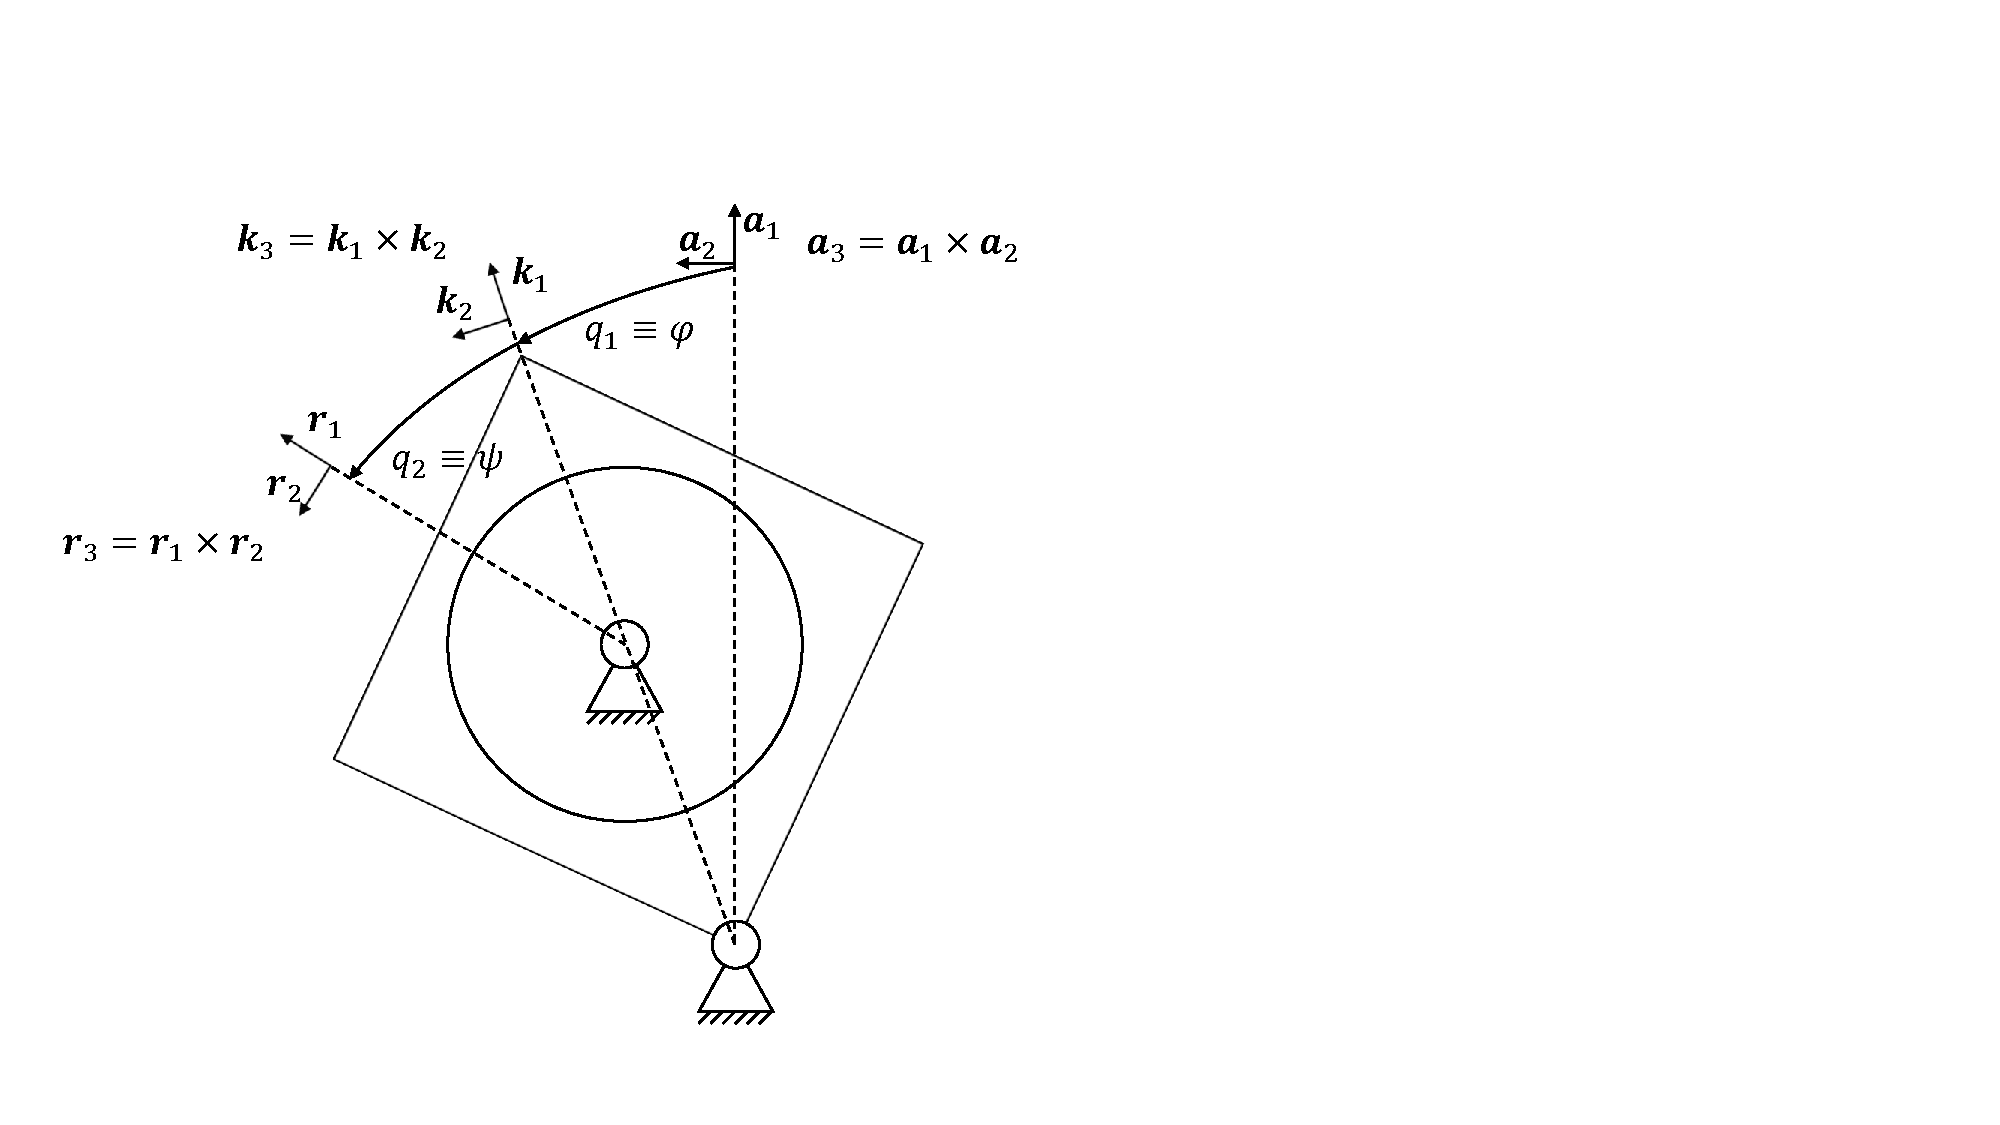
\includegraphics[width=0.6\linewidth, trim={1cm 1.5cm 18cm 3.5cm}, clip]{2_ModellWuerfelseite/img/ModellWuerfelseite}
\caption{Mechanischer Aufbau der Würfelseite, Quelle: eigene Darstellung}
\end{figure}

Zu Beginn werden der Untersuchung werden die Bezugssysteme festgelegt, welche durch drei, paarweise orthogonale, Einheitsvektoren definiert sind. Die Vektorbasis eines Bezugssystem dient als eine Art Einheit um vektorielle Größen, wie z.B. Position oder Geschwindigkeit, darzustellen. Das untersuchte System verfügt über das raumfeste Bezugssystem $A$, welches durch die drei Einheitsvektoren $\bs{a}_1$, $\bs{a}_2$ und $\bs{a}_3$ definiert wird. An der Würfelseite ist ein weiteres Bezugssystem $K$ fixiert, dessen Vektorbasis aus $\bs{k}_1$, $\bs{k}_2$ und $\bs{k}_3$ besteht. Zuletzt ist das, aus den Einheitsvektoren $\bs{r}_1$, $\bs{r}_2$ und $\bs{r}_3$ bestehende, Bezugssystem $R$ zu nennen, welches auf der Schwungmasse fixiert ist. 

Das holonome System verfügt über zwei rotatorische Freiheitsgrade, welche mit Hilfe der generalisierten Koordinaten $q_1 = \varphi$ und $q_2 = \psi$ beschrieben werden. Der Winkel $\varphi$ beschreibt die Rotation der Würfelseite um den Punkt $O$. Die Rotation der Schwungmasse $R$ relativ zu der Würfelseite wird von dem Winkel $\psi$ beschrieben. Mit Hilfe der generalisierten Koordinaten ist es möglich einen Vektor, welcher in einem Bezugssystem dargestellt ist, in ein zweites Bezugssystem zu projizieren. Als Beispiel soll die Position des Schwerpunktes von $K$ dienen, welche von dem Vektor $\bs{c}_K$ beschrieben wird. Mit Hilfe des Skalarproduktes eines Vektors mit einem Einheitsvektors, kann der Betrag des Vektors in Richtung des Einheitvektors ermittelt werden. Folglich können somit die Komponenten eines Vektors in einem beliebigen Bezugssystem dargestellt werden.

\begin{equation}
\bs{c}_K = \vecBS{K}{l_{AC}}{0}{0} = \vecBS{A}{\bs{c}_K \cdot \bs{a}_1}{\bs{c}_K \cdot \bs{a}_2} {\bs{c}_K \cdot \bs{a}_3} = \begin{pmatrix}
\bs{a}_1 \cdot \bs{k}_1 & \bs{a}_1 \cdot \bs{k}_2 & \bs{a}_1 \cdot \bs{k}_3 \\
\bs{a}_2 \cdot \bs{k}_1 & \bs{a}_2 \cdot \bs{k}_2 & \bs{a}_2 \cdot \bs{k}_3 \\
\bs{a}_3 \cdot \bs{k}_1 & \bs{a}_3 \cdot \bs{k}_2 & \bs{a}_3 \cdot \bs{k}_3 \\
\end{pmatrix} \cdot \bs{c}_K = \pMat{K}{A} \cdot \bs{c}_K
\end{equation}

Die Projektion kann somit in Form einer Matrix $\pMat{K}{A}$ dargestellt werden, welche aus den Skalarprodukten der Einheitsvektoren besteht. Die umgekehrte Projektion kann mit Hilfe der Matrix $\pMat{A}{K}$ durchgeführt werden, welche die Transponierte von $\pMat{A}{K}$ ist. Die Projektionsmatrizen des ursprünglichen Systems sind die folgenden.

\begin{equation}
\pMat{A}{K} = \begin{pmatrix}
c_{\varphi} && s_{\varphi} && 0 \\ -s_{\varphi} && c_{\varphi} && 0 \\ 0 && 0 && 1
\end{pmatrix} \hspace{15pt}
\pMat{K}{R} = \begin{pmatrix}
c_{\psi} && s_{\psi} && 0 \\ -s_{\psi} && c_{\psi} && 0 \\ 0 && 0 && 1
\end{pmatrix}
\end{equation}

Somit kann nun auch der Schwerpunkt der Würfelseite in dem raumfesten Bezugssystem $A$ dargestellt werden.

\begin{equation}
\bs{C}_K = \vecBS{K}{l_{AC}}{0}{0} = \presuper{A}{\begin{pmatrix}
\pMat{K}{A} \cdot \vecBS{K}{l_{AC}}{0}{0}
\end{pmatrix}} = \vecBS{A}{c_{\varphi} \cdot l_{AC}}{s_{\varphi} \cdot  l_{AC}}{0}
\end{equation}

An diesem Beispiel ist bereits zu erkennen, von welcher Bedeutung Bezugssysteme bei der Darstellung von Vektoren sind. Die Position des Schwerpunktes ist aus Sicht der Würfelseite konstant, jedoch ist seine Position im raumfesten Bezugssystem $A$ von dem Winkel $\varphi$ abhängig. Im Kehrschluss ist die Darstellung eines Vektors nur unter Angabe eines Bezugssystem sinnvoll.

Nachdem die Position bzw. Orientierung der Körper mit Hilfe der generalisierten Koordinaten bestimmt wurde besteht der nächste Schritt darin, die Geschwindigkeiten der beiden Körper zu bestimmen. Die Geschwindigkeit eines Körpers ist abhängig von dem Bezugssystem in welchem er sich bewegt. Folglich muss das Bezugssystem in wessen Relation sich ein Körper bewegt, bei der Darstellung der Geschwindigkeit berücksichtigt werden. Als Beispiel dient die Geschwindigkeit der Schwungmasse relativ zu der Würfelseite $\vel{K}{\bs{\omega}}{R}$, die Geschwindigkeit der Schwungmasse im raumfesten Bezugssystem $\vel{A}{\bs{\omega}}{R}$ und die Geschwindigkeit der Würfelseite in $A$, $\vel{A}{\bs{\omega}}{K}$.

\begin{equation}
\vel{K}{\bs{\omega}}{R} = \vecBS{A}{0}{0}{\dot{\psi}} \hspace{15pt} \vel{A}{\bs{\omega}}{K} = \vecBS{A}{0}{0}{\dot{\varphi}} \hspace{15pt} \vel{A}{\bs{\omega}}{R} = \vel{K}{\bs{\omega}}{R} + \vel{A}{\bs{\omega}}{K} = \vecBS{A}{0}{0}{\dot{\varphi}+\dot{\psi}}
\end{equation}

Es sei vermerkt, dass eine Geschwindigkeit in einem beliebigen Bezugssystem dargestellt werden kann, es handelt sich allerdings nach wie vor um die Geschwindigkeit des Körpers in dem ursprünglichen Bezugssystem, lediglich die Darstellung wurde verändert.

Um die Darstellung der Geschwindigkeiten zu vereinfachen, werden die generalisierten Geschwindigkeiten $u_1 \equiv \dot{\varphi}$ und $u_2 \equiv \dot{\psi}$ definiert. Somit ist es möglich die Geschwindigkeiten der Schwungmasse $\vel{A}{\bs{\omega}}{R}$ und der Würfelseite $\vel{A}{\bs{\omega}}{K}$ als Summe der generalisierten Geschwindigkeiten $u_i$ und der partiellen Geschwindigkeiten $\vel{A}{\bs{\omega}}{R}_i$ und $\vel{A}{\bs{\omega}}{K}_i$.

\begin{equation}
\vel{A}{\bs{\omega}}{K} = \dot{\varphi} \cdot \bs{a}_3 + \dot{\psi} \cdot 0 \hspace{5pt} \rightarrow \hspace{5pt} \vel{A}{\bs{\omega}}{K}_1 = \bs{a}_3 \hspace{15pt} \vel{A}{\bs{\omega}}{K}_2 = 0
\end{equation} 
\begin{equation}
\vel{A}{\bs{\omega}}{R} = \dot{\varphi} \cdot \bs{a}_3 + \dot{\psi} \cdot \bs{a}_3 \hspace{5pt} \rightarrow \hspace{5pt} \vel{A}{\bs{\omega}}{R}_1 = \bs{a}_3 \hspace{15pt}  \vel{A}{\bs{\omega}}{R}_2 = \bs{a}_3
\end{equation}

Bei den generalisierten Geschwindigkeiten $\dot{\varphi}$ und $\dot{\psi}$ handelt es sich um Skalare. Sie beschreiben die komponentenweise Zusammensetzung der Geschwindigkeiten der beiden Körper. Die partiellen Geschwindigkeiten hingegen sind Vektoren, welche die Orientierung der generalisierten Geschwindigkeiten wiedergeben und somit deren Beitrag zu der Bewegung in Richtung der Freiheitsgrade darstellen.

Der nächste Schritt besteht darin, die Drehmomente zu untersuchen, welche auf die Würfelseite und die Schwungmasse wirken. Mit Hilfe der wirkenden Kräfte können letzten Endes die Bewegungsgleichungen ermittelt werden.

Die Bewegung der Schwungmasse wird einerseits durch das Motormoment $\bs{T}^{R/M}_M$ beeinflusst, andererseits wird sie von der Reibung in $M$ durch das Drehmoment $\bs{T}^{R/M}_R$ verzögert. Das Reibmoment wird als proportional zur Geschwindigkeit $\dot{\psi}$ modelliert. Somit ergibt sich das resultierende Drehmoment $\bs{T}_R$.

\begin{equation}
\bs{T}^{R/M} = \bs{T}^{R/M}_M + \bs{T}^{R/M}_R = (T_M + C_{\psi} \cdot \dot{\psi})\cdot \bs{a}_3
\end{equation}

Das Motormoment $\bs{T}_M$ und das Reibmoment $\bs{R}_R$ wirken in umgekehrter Richtung auf die Würfelseite. Zusätzlich wird diese von dem Gravitationsmoment $\bs{T}^{K/O}_G$ und dem Reibmoment der Würfelseite $\bs{T}^{K/O}_R$. Aus der Summe dieser Komponenten ergibt sich das resultierende Drehmoment $\bs{T}^{K/O}$.

\begin{equation}
\bs{T}^{K/O} = \bs{T}^{K/O}_G - \bs{T}^{K/O}_R - \bs{T}^{R/M}_M + \bs{T}^{R/M}_R = 
(m_G \cdot g \cdot l_{AC} \cdot s_{\varphi} - C_{\varphi} \cdot \dot{\varphi} - T_M + C_{\psi} \cdot \dot{\psi}) \cdot \bs{a}_3
\end{equation}

Über das Skalarprodukt der resultierenden Drehmomente und der partiellen Geschwindigkeiten können die generalisierten aktiven Kräfte $F_1$ und $F_2$ berechnet werden. Diese stellen den Einfluss der wirkenden Kräfte und Momente auf die generalisierten Geschwindigkeiten $\dot{\varphi}$ und $\dot{\psi}$ dar.

\begin{equation}
F_1 = \vel{A}{\bs{\omega}}{K}_1 \cdot \bs{T}^{K/O} + \vel{A}{\bs{\omega}}{R}_1 \cdot \bs{T}^{R/M}= m_G \cdot g \cdot l_{AC} \cdot s_{\varphi} - C_{\varphi} \cdot \dot{\varphi}
\end{equation}
\begin{equation}
F_2 = \vel{A}{\bs{\omega}}{K}_2 \cdot \bs{T}^{K/O} + \vel{A}{\bs{\omega}}{R}_2 \cdot \bs{T}^{R/M}= T_M - C_{\psi} \cdot {\dot{\psi}}
\end{equation}

Die letztendlichen Bewegungsgleichungen werden über das Gleichgewicht der generalisierten, aktiven Kräfte und der generalisierten Trägheitskräfte gewonnen. Folglich muss zuletzt das Trägheitsmoment der Schwungmasse $\bs{T}^*_R$ und der Würfelseite $\bs{T}^*_K$ bestimmt werden. Ersteres ergibt sich aus dem Massenträgheitsmoment $I^{R/M}$ der Schwungmasse um den Punkt $M$ und seiner Winkelbeschleunigung in $A$.

\begin{equation}
\bs{T}^*_R = -I^{R/M} \cdot \vecBS{A}{0}{0}{\ddot{\varphi} + \ddot{\psi}}
\end{equation}

Das Trägheitsmoment der Würfelseite hängt von ihrer Winkelbeschleunigung in $A$,ihrem Massenträgheitsmoment $I^{K/O}$ um $O$ und der Position bzw. dem Gewicht der Schwungmasse ab.

\begin{equation}
\bs{T}^*_K = -(I^{K/O} + m_R \cdot l_{AB}^2) \cdot \vecBS{A}{0}{0}{\ddot{\varphi}}
\end{equation}

Die generalisierten Trägheitskräfte $F^*_1$ und $F^*_2$ ergeben sich wiederum durch die Skalarmuliplikation mit den partiellen Geschwindigkeiten. Das heißt die Trägheitsmomente der beiden Körper werden in die Bewegungsrichtung der generalisierten Geschwindigkeiten, also der Freiheitsgrade, projiziert.

\begin{equation}
F^*_1 = \vel{A}{\omega}{K}_1 \cdot \bs{T}^*_K + \vel{A}{\omega}{R}_1 \cdot \bs{T}^*_R = -(I^{K/O} + I^{R/M} + m_R \cdot l_{AB}^2)\cdot \ddot{\varphi} - I^{R/M} \cdot \ddot{\psi}
\end{equation}
\begin{equation}
F^*_2 = \vel{A}{\omega}{K}_2 \cdot \bs{T}^*_K + \vel{A}{\omega}{R}_2 \cdot \bs{T}^*_R = -I^{R/M}\cdot(\ddot{\varphi}+\ddot{\psi})
\end{equation}

Die Bewegungsgleichungen ergeben sich nun aus der Summe der generalisierten aktiven Kräften $F_i$ und der generalisierten Trägheitskräfte $F^*_i$. Die Aussage dieser Gleichungen besteht darin, dass die Projektion, der wirkenden Kräfte in Richtung der partiellen Geschwindigkeiten, gleich der Projektion der Impulsänderung in Richtung der partiellen Geschwindigkeiten ist.

\begin{equation}
F_1 + F^*_1 = 0 \hspace{5pt} \rightarrow \hspace{5pt} (I^{K/O}+I^{R/M}+m_R\cdot l_{AB}^2)\cdot \ddot{\varphi} = m_G \cdot g \cdot l_{AC} \cdot s_{\varphi} - C_{\varphi} \cdot \dot{\varphi} - I^{R/M} \cdot \ddot{\psi}
\end{equation}
\begin{equation}
F_2 + F^*_2 = 0 \hspace{5pt} \rightarrow \hspace{5pt} I^{R/M} \cdot \ddot{\psi} = T_M - C_{\psi} \cdot \dot{\psi} - I^{R/M} \cdot \ddot{\varphi}
\end{equation}

\subsection{Zustandsraumdarstellung}
Ein beliebiges Differentialgleichungssystem kann in ein System von Differentialgleichungen 1. Ordnung transformiert werden. Dadurch lässt sich die so genannte Zustandsraumdarstellung bestimmen, welche erhebliche Vorteile in der Systemanalyse und dem bei Reglerentwurf mit sich bringt. Ausgangspunkt zur Bestimmung dieser Darstellung ist die Definition des Zustandvektors $\bs{x}$. Für die Würfelseite wird folgende Definition verwendet.
\begin{equation}
\bs{x} = \begin{pmatrix}
x_1 \\ x_2 \\ x_3
\end{pmatrix} \equiv \begin{pmatrix}
\varphi \\ \dot{\varphi} \\ \dot{\psi}
\end{pmatrix}
\end{equation}

Mit Hilfe der Zustände können die linearisierten Bewegungsgleichungen in ein System aus drei Differentialgleichungen erster Ordnung umgeschrieben werden. Zusätzlich muss hierfür der Eingangsvektor $\bs{u}$ definiert werden, der in diesem Fall lediglich aus dem Motormoment $T_M$ besteht.
\begin{equation}
u \equiv T_M
\end{equation}
\begin{equation}
\begin{split}
\dot{x_1} &= x_2 \\
\dot{x_2} &= \frac{m_G \cdot g \cdot l_M \cdot x_1 - C_{\varphi}\cdot x_2 + C_{\psi} - u }{I^{K/O}+m_r\cdot l^2_{M}} \\
\dot{x_3} &= \frac{I^{G/O}\cdot(T_M - C_{\psi}\cdot x_3)}{I^{R/M}(I^{K/O}+m_R\cdot l^2_{M})}-\frac{m_G\cdot g \cdot l_C \cdot x_1 - C_{\varphi}\cdot x_2}{I^{K/O}+m_r \cdot l^2_M}
\end{split}
\end{equation}

Dieses Gleichungssystem lässt sich in die folgende, vektorielle Form umschreiben, welche die erste Gleichung der Zustandsraumdarstellung ist.

\begin{equation}
\dot{\bs{x}}=\bs{A}\cdot \bs{x}+\bs{B}\cdot \bs{u}
\end{equation}
\begin{equation}
\bs{A} = \begin{pmatrix}
 0 & 1 & 0 \\
 \frac{m_G\cdot g\cdot l_C}{I^{K/O}+m_r\cdot l^2_M} & 
 \frac{-C_{\varphi}}{I^{K/O}+m_r\cdot l^2_M} &
 \frac{C_{\psi}}{I^{K/O}+m_r\cdot l^2_M} \\
 \frac{-m_G\cdot g \cdot l_C}{I^{K/O}+m_r\cdot l^2_M} &
 \frac{C_{\varphi}}{I^{K/O}+m_r\cdot l^2_M} &
 \frac{C_{\psi}}{I^{G/O}(I^{K/O}+m_r\cdot l^2_M)}
\end{pmatrix}
\hspace{35pt}
\bs{B} = \begin{pmatrix}
0 \\ \frac{1}{I^{K/O}+m_r\cdot l^2_M} \\ \frac{I^{G/O}}{I^{R/M}(I^{K/O}+m_r \cdot l^2_M}
\end{pmatrix}
\end{equation}

Die Matrizen $\bs{A}$ und $\bs{B}$ heißen System- bzw. Eingangsmatrix und stellen den Zusammenhang zwischen des Zustand- und Eingangsvektors zu der zeitlichen Änderung des Zustandvektors dar.
Im nächsten Schritt wird der Ausgangsvektor $\bs{y}$ definiert. Hierfür werden die Ausgangsmatrix $\bs{C}$ und die Durchgangsmatrix $\bs{D}$ bestimmt, welche den Einfluss des Zustands- und Eingangsvektors auf die Ausgangsgrößen wiedergeben. In dem Fall der Würfelseite primär der Ausfallwinkel $\varphi$ geregelt werden, welcher somit als Ausgangsgröße aufgeführt wird. Zusätzlich soll die Geschwindigkeit der Schwungmasse $\dot{\psi}$ minimiert werden, weshalb diese Größe ebenfalls im Ausgangsvektor enthalten ist. einzige Ausgangsgröße dar.
\begin{equation}
\bs{y} = \begin{pmatrix}
\varphi \\ \dot{\psi}
\end{pmatrix}
\end{equation}
\begin{equation}
\bs{y} = \bs{C} \cdot \bs{x} + \bs{D} \cdot \bs{u}
\end{equation}
\begin{equation}
\bs{C} = \begin{pmatrix}
1 & 0 & 0 \\ 0 & 0 & 1
\end{pmatrix}
\hspace{35pt}
\bs{D} = \begin{pmatrix}
0
\end{pmatrix}
\end{equation}
Als nächstes stellt sich die Frage, wie aus der Zustandsraumdarstellung die Lösung der Bewegungsgleichungen bestimmt werden können. Hierfür kann nach (RT2, S.6 ff.) der Exponentialansatz für einzelne Differentialgleichungen auf die vektorielle Zustandsraumdarstellung übertragen werden.
\begin{equation}
\bs{x} = e^{\bs{A}\cdot t} \cdot \bs{x}_0 + \int^t_0 e^{\bs{A}(t - \tau)} \bs{B}\cdot \bs{u}(\tau) d\tau
\end{equation}
Die Matrix-Exponentialfunktion $e^{\bs{A}\cdot t}$ heißt Fundamentalmatrix $\Phi(t)$. Für die Herleitung der folgenden Definition sei ebenfalls auf (RT2, S.6 ff.) verwiesen.
\begin{equation}
\Phi(t) = e^{\bs{A}\cdot t} = \sum^{\infty}_{k=0} \bs{A}^k \cdot \frac{t^k}{k!}
\end{equation}
Mit Hilfe der Fundamentalmatrix kann einerseits die homogene Lösung $\bs{x}_h$ des Zustandraums bestimmt werden.
\begin{equation}
\bs{x}_h(t) = \Phi(t)\cdot \bs{x}_0 \hspace{35pt} \vert \hspace{15pt} \bs{x}_0 = \bs{x}(t=0)
\end{equation}
Diese die Eigenbewegung des Systems, welche von den Anfangswerten der Zustände abhängt. Andererseits kann die partikuläre Lösung $\bs{x}_p$ berechnet werden, welche die, durch die Eingangsgrößen verursachte, Systembewegung wiedergibt.
\begin{equation}
\bs{x}_p(t) = \int^t_0 \Phi(t-\tau)\cdot \bs{B}\cdot \bs{u}(\tau)d\tau
\end{equation}
Neben dem Verlauf der Zustandsvektors $\bs{x}$ spielt der Zusammenhang der Eingangs- und Ausgangsgrößen eine zentrale Rolle. Dieser wird von der Übertragungsfunktion $g(t)$ bzw., bei Mehrgrößensystemen, der Übertragungsmatrix $\bs{G}(t)$ beschrieben.
Die zweite Gleichung der Zustandsraumdarstellung führt zu dem Verlauf des Ausgangvektors $\bs{y}(t)$. Setzt man die Lösung für $\bs{x}(t)$ ein ergibt sich:
\begin{equation}
\bs{y}(t) = \bs{C}\Phi(t)\bs{x}_0 + \int^t_0 \bs{C}\Phi(t-\tau)\bs{B}\bs{u}(\tau)d\tau
\end{equation}
Durch die folgende Definition der Übertragungsmatrix $\bs{G}(t)$ lässt sich diese Gleichung weiter vereinfachen.
\begin{equation}
\bs{y}(t) = \bs{C}\Phi(t)\bs{x}_0 + \int^t_0 \bs{G}(t-\tau)\bs{u}(\tau)d\tau \hspace{35pt} \vert \hspace{15pt} \bs{G}(t) = \bs{C}\Phi(t)\bs{B}+\bs{D}\delta(t)
\end{equation}
Die Lösung des Ausgangvektors setzt sich ebenfalls aus der homogenen Lösung
\begin{equation}
\bs{y}_h(t) = \bs{C}\Phi(t)\bs{x}_0
\end{equation}
und der partikulären Lösung, welche sich aus dem Faltungsintegral der Übertraungsmatrix und des Eingangsvektors ergibt.
\begin{equation}
\bs{y}_p(t) = \int^t_0 \bs{G}(t-\tau)\bs{u}(\tau)d\tau = \bs{G}(t)*\bs{u}(t)
\end{equation}
Die obigen Darstellungen zeigen, dass mit Hilfe der Fundamental- und Übergangsmatrix sowohl die homogenen als auch partikulären Lösungen des Zustands- und Ausgangsvektors berechnet werden können. Das bedeutet, dass sie das vollständige Systemverhalten wiedergeben. Deshalb sollen im nächsten Schritt weitere Methoden untersucht werden um die beiden Matrizen zu ermitteln.

Durch die Laplace-Transformation der Zustandsraumdarstellung ergeben sich die folgenden Gleichungen im Bildbereich.
\begin{equation}
s\bs{X}(t) - \bs{x}_0 = \bs{A}\bs{X}(s) + \bs{B}\bs{U}(s)
\end{equation}
\begin{equation}
\bs{Y}(s) = \bs{C}\bs{X}(s)+\bs{D}\bs{U}(s)
\end{equation}
Aus der ersten Gleichung lässt sich die Lösung des Zustandvektors im Bildbereich ermitteln.
\begin{equation}
\bs{X}(s) = (s\cdot \bs{I} - \bs{A})^{-1}\bs{x}_0 + (s\cdot\bs{I}-\bs{A})^{-1}\bs{B}\bs{U}(s)
\end{equation}
Vergleicht man diese Gleichung mit der Lösung im Zeitbereich so ergibt sich für die Laplace-Transformierte der Fundamentalmatrix:
\begin{equation}
\mathcal{L}(\Phi(t)) = \bs{\Phi}(s) = (s\cdot\bs{I}-\bs{A})^{-1}
\end{equation}
Somit kann nun auch die Übertragungsmatrix im Bildbereich berechnet werden.
\begin{equation}
\mathcal{L}(\bs{G}(t)) = \bs{G}(s) = \bs{C}\bs{\Phi}(s)\bs{B}+\bs{D}
\end{equation}
Mit Hilfe der Berechnungsvorschriften im Bildbereich können nun auch die Fundamental- und Übertragungsmatrix der Würfelseite bestimmt werden. Es sei allerdings angemerkt, dass die Berechnung, welche im Vergleich zu den Vorschriften im Zeitbereich relativ einfach ist, nur mit Hilfe von Hilfsmitteln wie MATLAB durchzuführen ist. Auch die Darstellung der symbolischen Wert führt zu kaum interpretierbaren Ergebnissen, weshalb die ermittelten Werte für die Systemgrößen verwendet werden.
\begin{equation}
\bs{\Phi}(s) = \begin{pmatrix}

\end{pmatrix}
\end{equation}
\begin{equation}
\bs{G}(s)= \begin{pmatrix}
\frac{17,0}{s+9,7}+\frac{-16,0}{s-7,9}+\frac{-1,0}{s+0,3} \\
\frac{169,8}{s+9,7}+\frac{122,1}{s-7,9}+\frac{8558,6}{s+0,3}
\end{pmatrix}
\end{equation}
In den Darstellung ist leicht zu erkennen, dass das System über Pole verfügt, welche in der rechten Halbebene liegen, und somit instabil ist. 

\section{Sensorik}
Für die Berechnung des Regelkreises müssen die Zustandsgrößen erfasst erfasst werden, deshalb beschäftigt sich der folgende Abschnitt mit der verwendeten Sensorik und derer Auswertung. Hierfür müssen die Sensoren in das mechanische Modell eingebunden werden um Messkennlinien zu bestimmen. Hierbei zeigt sich, dass mehrere Möglichkeiten bestehen die verschiedenen Größen zu ermitteln. Eine Vorarbeit hat gezeigt, dass diese von unterschiedlichen Störungen betroffen sind, weshalb Methoden erarbeitet werden müssen um einen qualitativen Vergleich zu ermöglichen. 

\begin{figure}[!h]
\centering
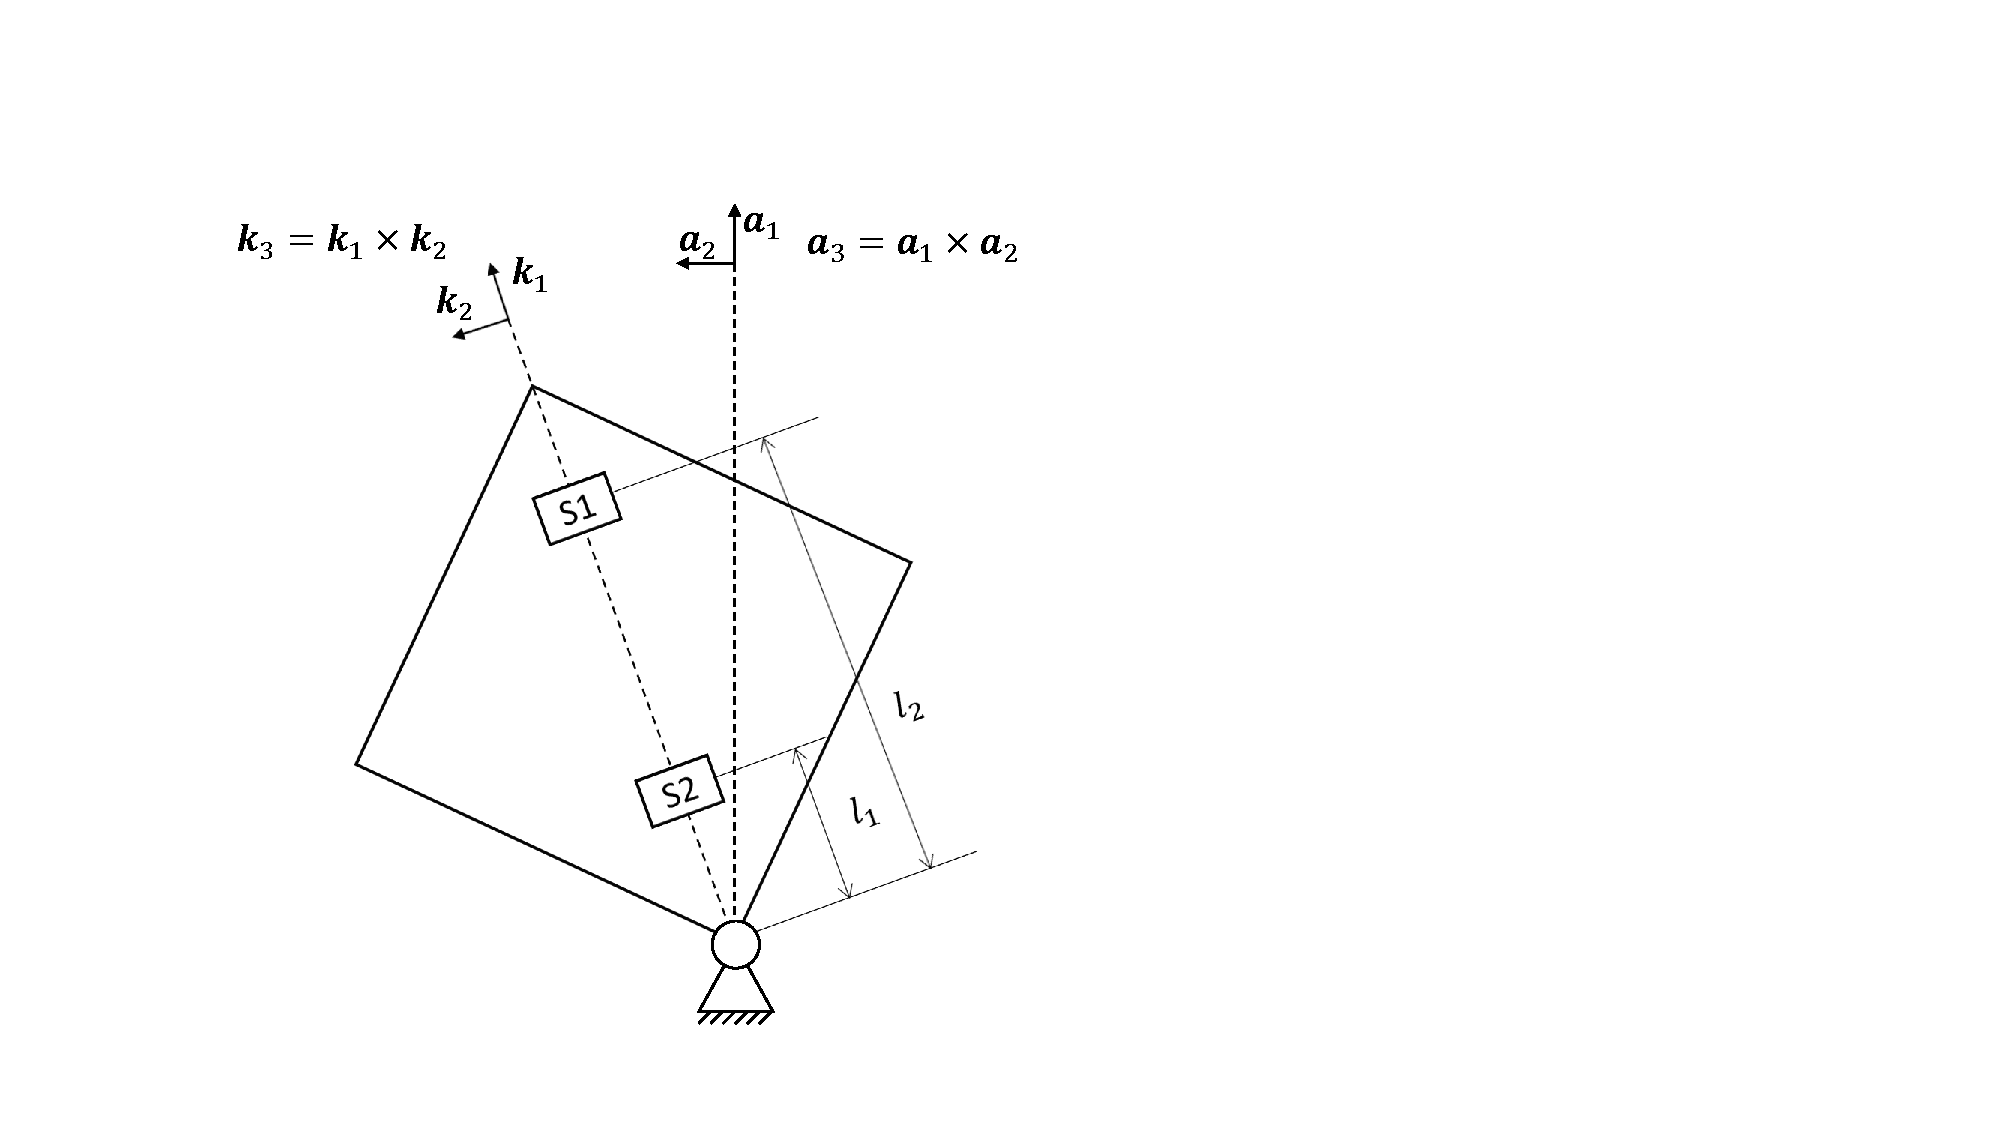
\includegraphics[width=0.6\linewidth, trim={1cm 1.5cm 18cm 3.5cm}, clip]{3_Sensorik/img/SensorAnordnung}
\caption{Anordnung der Sensoren an der Würfelseite, Quelle: eigene Darstellung}
\end{figure}

An der Würfelseite sind zwei MPU6050-ICs angebracht, um die Größen $\varphi$, $\dot{\varphi}$ und $\ddot{\varphi}$ zu messen. Die ICs verfügen über einen Beschleunigungs- und Drehratensensor, welche jeweils Messwerte in Richtung von drei Achsen liefern. Zuerst müssen Messkennlinien ermittelt werden. Das heißt die Messwerte der Sensoren werden mit Hilfe des mechanischen Modells in Zusammenhang mit den Messgrößen $\varphi$, $\dot{\varphi}$ und $\ddot{\varphi}$ gebracht. 

Die Messwerte der Drehratensensoren entsprechen der Winkelgeschwindigkeit der Würfelseite im körperfesten Bezugssystem $K$.

\begin{equation}
\bs{\omega}_{S_i} = \begin{pmatrix}
\omega^{S_i}_x \\ \omega^{S_i}_y \\ \omega^{S_i}_z
\end{pmatrix} = \presuper{K}{\big(\vel{A}{\omega}{K}\big)} = \begin{pmatrix}
{0} \\ {0} \\ {\dot{\varphi}}
\end{pmatrix}
\end{equation}

Somit sind nur die Komponenten in Richtung der Z-Achse von Bedeutung. Diese werden als Messwerte $y_i$ definiert.

\begin{equation}
y_i \equiv \omega^{S_i}_z \hspace{35pt} y_i = \dot{\varphi} \hspace{35pt} (i=1, 2)
\end{equation}

Die Ausgabewerte $\bs{a}_{S_i}$ der Beschleunigungssensoren setzt sich, nach dem idealisierten Modell, aus zwei Termen zusammen. Der erste Term entspricht der Beschleunigung der Sensoren im raumfesten Bezugssystem $A$, welche gleich der zweiten Ableitung des Ortvektors $\bs{s}_i$ der Sensoren mit Respekt zu $A$ ist.

\begin{equation}
\begin{split}
\vel{A}{a}{S_i} &= \frac{\presuper{A}{d} \vel{A}{v}{S_i}}{dt} = \frac{\presuper{A}{d}}{dt}\big(\vel{A}{\bs{\omega}}{K} \times \bs{s}_i\big) = \frac{\presuper{A}{d}\vel{A}{\omega}{K}}{dt}\times \bs{s}_i + \vel{K}{\omega}{S_i} \times \frac{\presuper{A}{d}\bs{s}_i}{dt} \\
&= \vel{K}{\alpha}{S_i} \times \bs{s}_i + \vel{A}{\omega}{K} \times \big(\vel{A}{\omega}{K} \times \bs{s}_i\big)
\\
&= \vecBS{K}{0}{0}{\ddot{\varphi}} \times \vecBS{K}{l_i}{0}{0}  + \vecBS{K}{0}{0}{\dot{\varphi}} \times \begin{pmatrix}
\vecBS{K}{0}{0}{\dot{\varphi}} \times \vecBS{K}{l_i}{0}{0} 
\end{pmatrix} = \vecBS{K}{-\dot{\varphi}^2 \cdot l_i}{\ddot{\varphi}\cdot l_i}{0}
\end{split}
\end{equation}

Der zweite Term wird von der Gravitation beeinflusst. Das heißt er entspricht der Darstellung des Erdbeschleunigungsvektors im körperfesten Bezugssystem $K$.

\begin{equation}
\bs{g} = \pMat{A}{K} \cdot \vecBS{A}{-g}{0}{0} = \vecBS{K}{-g \cdot c_{\varphi}}{g \cdot s_{\varphi}}{0}
\end{equation}

Somit ergeben sich die folgenden Zusammenhänge für die Anzeigewerte $\bs{a}_{S_i}$ der Beschleunigungssensoren, welche wiederum als Messwerte $y_3,...,y_6$ definiert werden.

\begin{equation}
\bs{a}_{S_i} = \begin{pmatrix}
\ddot{x}_{S_i} \\ \ddot{y}_{S_i} \\ \ddot{z}_{S_i}
\end{pmatrix} = 
\presuper{K}{\big(\vel{A}{a}{S_i} + \bs{g}\big)} = \vecBS{K}{-\dot{\varphi}^2 \cdot l_i - g\cdot c_{\varphi}}{\ddot{\varphi}\cdot l_i + g \cdot s_{\varphi}}{0}
\end{equation}
\begin{equation}
\begin{split}
&y_3 \equiv a^{S_1}_x \hspace{35pt} y_3 = -\dot{\varphi}^2 \cdot l_1 - g \cdot c_{\varphi} \\
&y_4 \equiv a^{S_2}_x \hspace{35pt} y_4 = -\dot{\varphi}^2  \cdot l_2 - g\cdot c_{\varphi} \\
&y_5 \equiv a^{S_1}_y \hspace{35pt} y_5 = \ddot{\varphi} \cdot l_1 + g\cdot s_{\varphi} \\
&y_6 \equiv a^{S_2}_y \hspace{35pt} y_6 = \ddot{\varphi} \cdot l_2 + g\cdot s_{\varphi}
\end{split}
\end{equation}

\subsection{Untersuchung der Messsysteme für  $\dot{\varphi}$}
Die Winkelgeschwindigkeit der Würfelseite kann mit Hilfe der beiden Drehratensensoren gemessen werden. Da zwei dieser Sensoren verwendet werden kann ein dritter Messwert definiert werden, welcher der Mittlung der beiden Sensorwerte entspricht.
\begin{equation}
\begin{split}
y_1 \equiv \omega^{S_1}_z & y_1 = \dot{\varphi} \\
y_2 \equiv \omega^{S_2}_z & y_2 = \dot{\varphi} \\
y_3 \equiv \frac{y_1+y_2}{2} & y_3 = \dot{\varphi}
\end{split}
\end{equation}
Die drei Messsysteme besitzen die selbe Kennlinie und somit identische Empfindlichkeit, weshalb diese nicht als Bewertungskriterium verwendet werden kann. Allerdings können die Messwerte in der Ruhelage über einen Zeitraum $T$ aufgenommen werden. In dieser Messreihe verschwindet der Wert der Messgröße $\dot{\varphi}=0$. Deshalb handelt es sich bei den gemessenen Werten um reine Rauschsignale, derer Effektivwerte bestimmt werden können. Diese sollen als erstes Bewertungskriterium verwendet werden.
Aus der Messreihe über $n=8096$ Werte bei einer Abtastfrequenz $f_a=50Hz$ ergeben sich die folgenden Effektivwerte.
\begin{equation}
\begin{split}
R^{Eff}_1 &= \sqrt{\frac{1}{n}\sum^n_{k=1}{y_1(k)}^2} = 0.0010 \\
R^{Eff}_2 &= \sqrt{\frac{1}{n}\sum^n_{k=1}{y_2(k)}^2} = 0.0010 \\
R^{Eff}_3 &= \sqrt{\frac{1}{n}\sum^n_{k=1}{y_3(k)}^2} = 0.0007
\end{split}
\end{equation}
Der Effektivwert des Rauschens wird durch die Mittelung der beiden Sensorwerte minimiert. Deshalb wird der Messwert $y_3$ zur Bestimmung von $\dot{\varphi}$ verwendet.

\subsection{Ermittlung von $\varphi$}
Zuerst sollen die Möglichkeiten zur Bestimmung von $\varphi$ näher untersucht werden. Die Kennlinien der Beschleunigungssensoren zeigen, dass die momentane Ausrichtung der Würfelseite deren Anzeigewerte beeinflusst. Allerdings hängen die Beschleunigungswerte von weiteren Messgrößen ab, weshalb ein einzelner Wert nicht ausreicht um den Winkel $\varphi$ zu berechnen. Allerdings kann durch die gewichtete Differenz zweier Beschleunigungswerte der Einfluss der Winkelgeschwindigkeit und -beschleunigung eliminiert werden.
\begin{equation}
\begin{split}
y_9 \equiv y_3 - \frac{l_1}{l_2}y_4 &y_9 = -g\cdot c_{\varphi}\cdot (1-\frac{l_1}{l_2}) \\
y_{10} \equiv y_5 - \frac{l_1}{l_2}y_6 &y_{10} = g\cdot s_{\varphi}\cdot(1-\frac{l_1}{l_2}) \\
y_{11}\equiv \frac{y_{10}}{y_{11}} &y_{11} = -tan(\varphi)
\end{split}
\end{equation}
Als erstes Beurteilungskriterium werden die Empfindlichkeiten der Messsysteme verwendet, welche sich durch die partielle Ableitung der Kennlinien nach der Messgröße ergeben.
\begin{equation}
\begin{split}
S_9(\varphi) &= \frac{\partial y_9}{\partial \varphi} = g\cdot s_{\varphi}\cdot (1 - \frac{l_1}{l_2}) \\
S_{10}(\varphi) &= \frac{\partial y_{10}}{\partial \varphi} = g \cdot c_{\varphi} \cdot (1- \frac{l_1}{l_2}) \\
S_{11}(\varphi) &= \frac{\partial y_{11}}{\partial \varphi} = -tan(\varphi)^2 - 1
\end{split}
\end{equation}
\begin{figure}[h!]
\centering
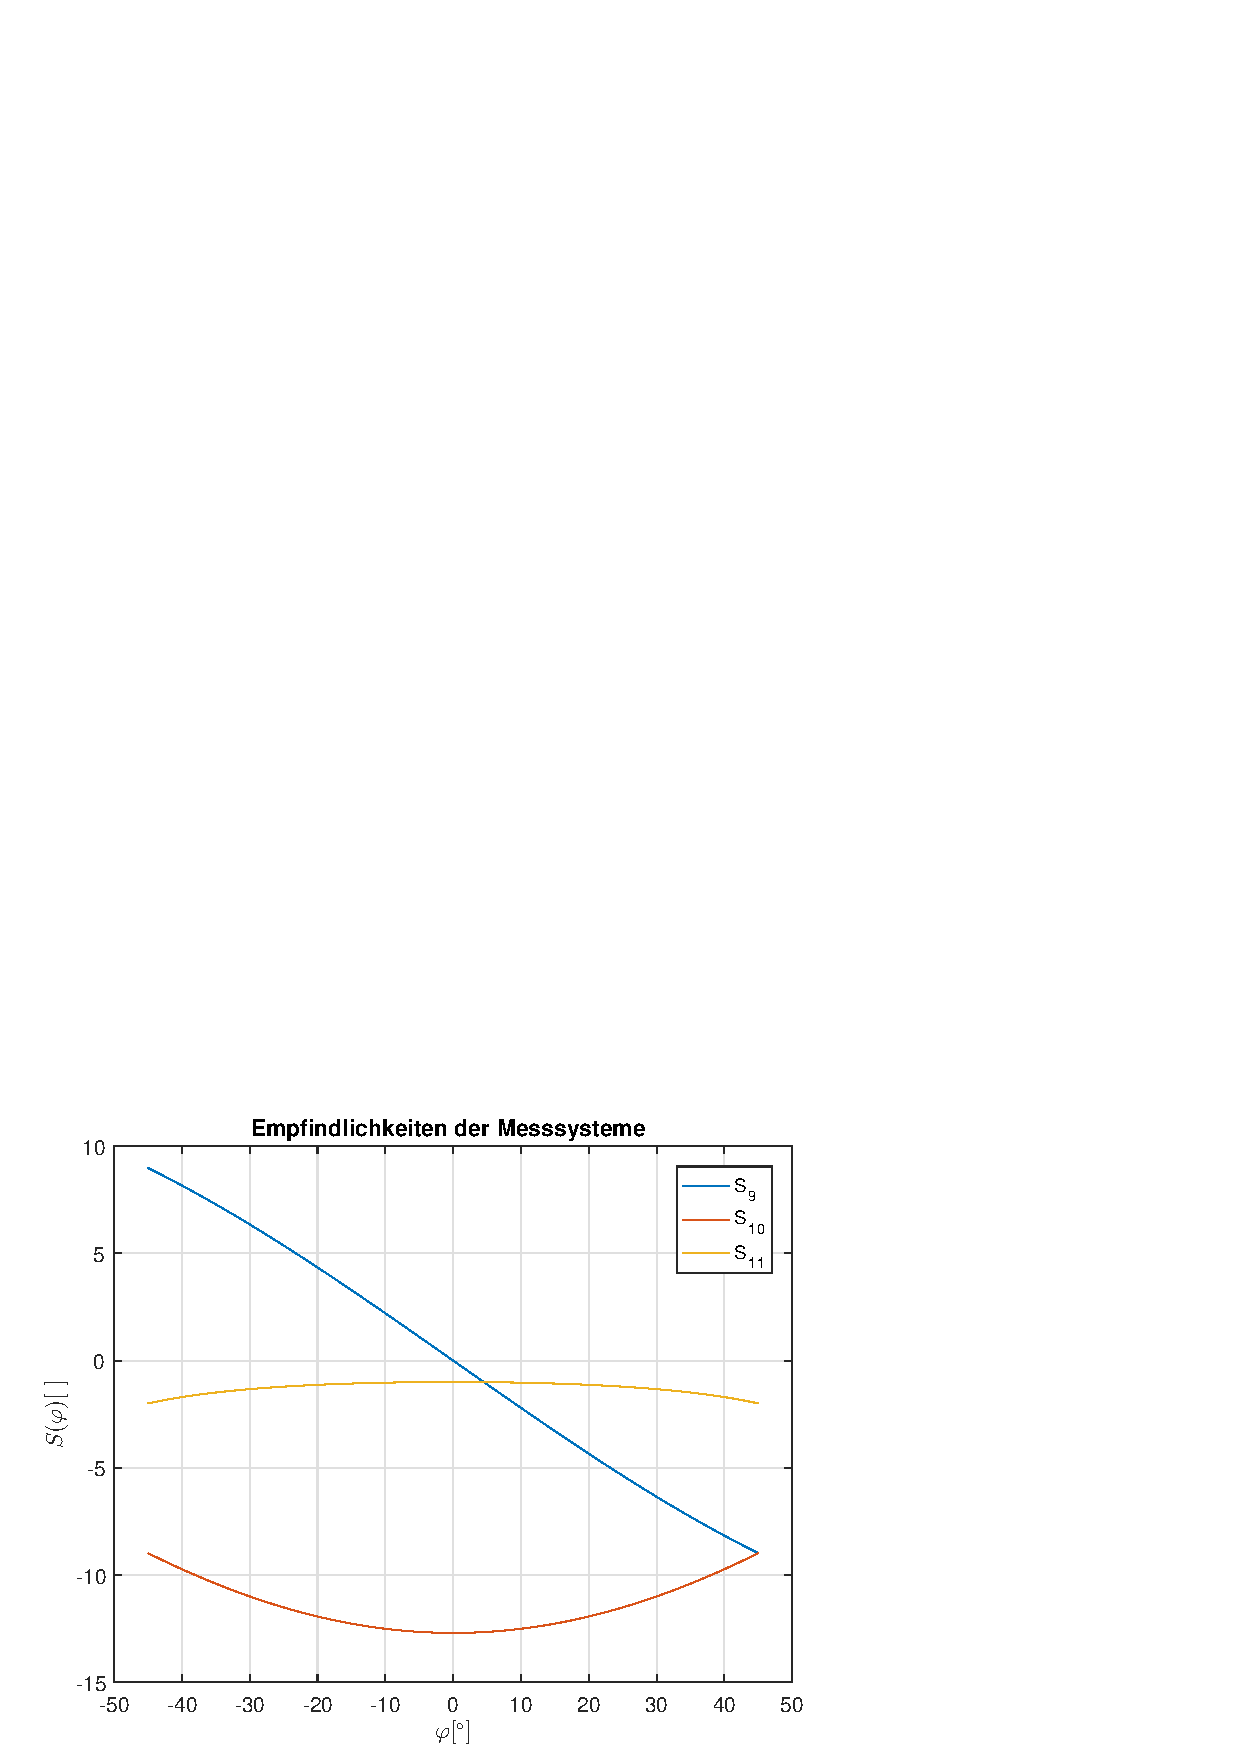
\includegraphics[width=0.5\linewidth]{3_Sensorik/img/empfindlichkeit_phi}
\caption{Empfindlichkeiten für $\varphi$, Quelle: eigene Darstellung}
\end{figure}
In der Abbildung ist deutlich zu erkennen, dass der Messwert $y_{10}$ die höchste Empfindlichkeit besitzt. Hieraus folgt, dass bereits kleine Änderung der Messgröße zu einer deutlichen Änderung des Messwertes führen. Folglich ist zu erwarten, dass das Signal-Rausch-Verhältnis mit zunehmender Empfindlichkeit größer wird.
Um die Signal-Rausch-Verhältnisse der Messsysteme zu bestimmen, wird die Würfelseite in einer bekannten Ausrichtung fixiert. Dadurch entsteht ein stationärer Prozess und es kann angenommen werden, dass der Mittelwert des Signales dem Nutzsignal entspricht. Die folgende Abbildung zeigt den Verlauf der Messgröße $\varphi$ aus den drei Messsystemen.

\begin{figure}[h!]
\centering
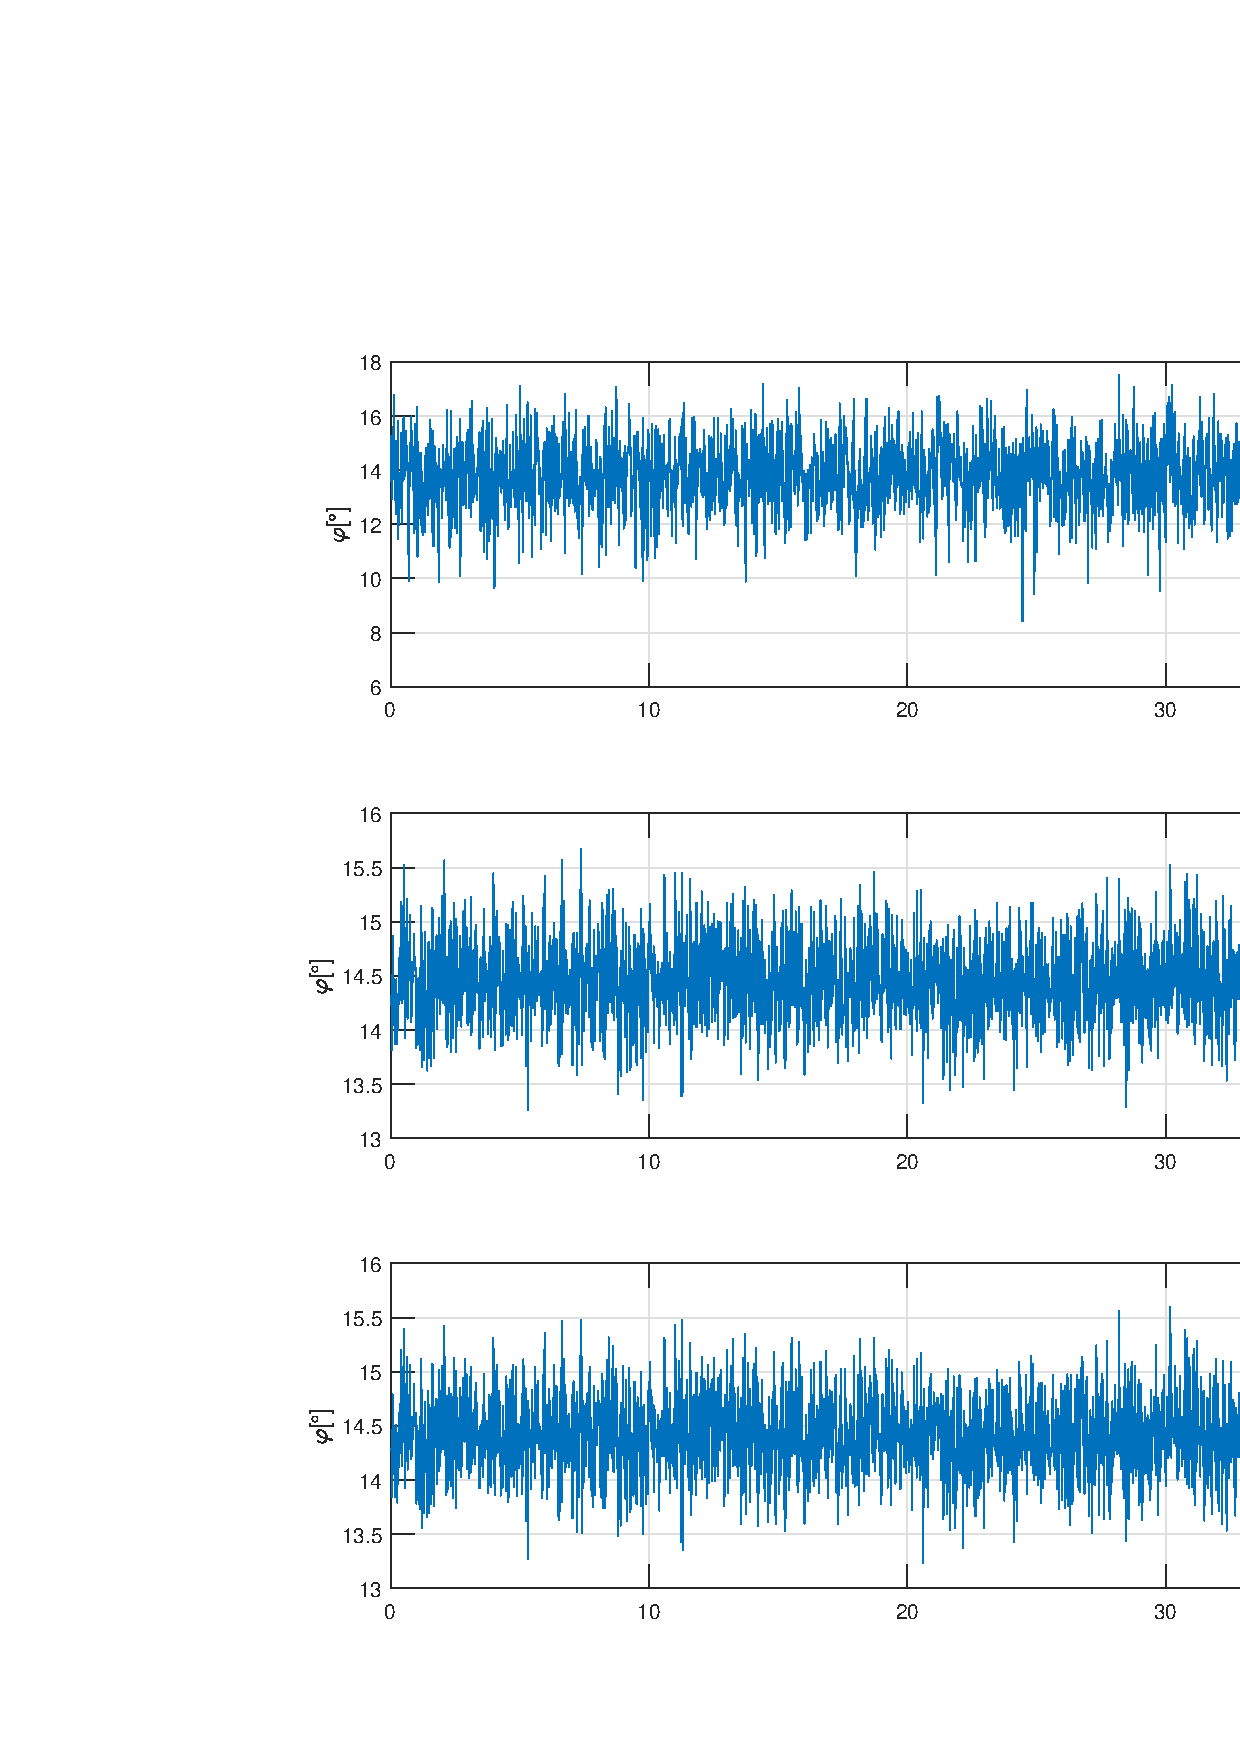
\includegraphics[width=\linewidth]{3_Sensorik/img/snr_phi_plot}
\caption{Signal-Rausch-Verhältnis der $\varphi$-Messsysteme, Quelle: eigene Darstellung}
\end{figure}

Die resultierenden Signal-Rausch-Verhältnisse sind:
\begin{equation}
SNR(y_9) = 20.57dB \hspace{35pt}  SNR(y_{10}) = 31.21dB \hspace{35pt} SNR(y_{11})=31.50dB
\end{equation}

Hier zeigt sich, dass das SNR von $y_{11}$ trotz niedriger Empfindlichkeit am höchsten ist. Einen mögliche Ursache hierfür ist, dass es sich bei dem Rauschen nicht um rein zufällige Signale handelt sondern diese von Störeinflüssen wie z.B. der Temperatur abhängen. Die Temperatur fließt nach Hersteller als weitere Proportionalität in die Kennlinie ein und wird somit durch die Division zweier mehrere Messwerte gekürzt. Weshalb die Division der beiden Messwerte zu einem verbesserten Signal-Rausch-Verhältnis führt.
In einer Vorarbeit hat sich herausgestellt, dass die Winkelschätzung aus den Beschleunigungssensoren bei hochfrequenten Anregungen von starken Störungen betroffen sind. Deshalb wird neben 
Neben den Beschleunigungssensoren kann der Winkel $\varphi$ auch aus den integrierten Winkelgeschwindigkeiten berechnet werden. Somit ergeben sich die beiden Schätzungen für den Winkel $\varphi$.
\begin{equation}
\varphi_A = -atan(y_{11}) \hspace{35pt} \varphi_G = \int y_3 dt
\end{equation}
Um die bereits angesprochen Störungen der Beschleunigungssensoren bei hochfrequenter Anregung zu untersuchen werden im nächsten Schritt Schwingversuche durchgeführt. Hierfür wird die Würfelseite als gewöhnliches Pendel aufgehängt, wodurch sich das Vorzeichen des Gravitationsmomentes ändert. Somit ergibt sich die folgende Zustandsraumdarstellung.

\begin{equation}
\dot{\bs{x}}=\bs{A}\cdot \bs{x}+\bs{B}\cdot \bs{u}
\end{equation}
\begin{equation}
\bs{A} = \begin{pmatrix}
 0 & 1 & 0 \\
 \frac{-m_G\cdot g\cdot l_C}{I^{K/O}+m_r\cdot l^2_M} & 
 \frac{-C_{\varphi}}{I^{K/O}+m_r\cdot l^2_M} &
 \frac{C_{\psi}}{I^{K/O}+m_r\cdot l^2_M} \\
 \frac{m_G\cdot g \cdot l_C}{I^{K/O}+m_r\cdot l^2_M} &
 \frac{C_{\varphi}}{I^{K/O}+m_r\cdot l^2_M} &
 \frac{C_{\psi}}{I^{G/O}(I^{K/O}+m_r\cdot l^2_M)}
\end{pmatrix}
\hspace{35pt}
\bs{B} = \begin{pmatrix}
0 \\ \frac{1}{I^{K/O}+m_r\cdot l^2_M} \\ \frac{I^{G/O}}{I^{R/M}(I^{K/O}+m_r \cdot l^2_M}
\end{pmatrix}
\end{equation}

\begin{equation}
\bs{y} = \begin{pmatrix}
\varphi
\end{pmatrix}
\end{equation}
\begin{equation}
\bs{y} = \bs{C} \cdot \bs{x} + \bs{D} \cdot \bs{u}
\end{equation}
\begin{equation}
\bs{C} = \begin{pmatrix}
1 & 0 & 0 
\end{pmatrix}
\hspace{35pt}
\bs{D} = \begin{pmatrix}
0
\end{pmatrix}
\end{equation}

Mit Hilfe der Zustandsraumdarstellung kann die Übertragungsfunktion $G(s)$ im Bildbereich berechnet werden.s

\section{Herleitung/Interpretation Fourier-Spektren}
Die Beurteilung der dynamischen Störungen erfolgt über eine Spektralanalyse. Hierfür wird die DFT der Messgrößen berechnet. Um die Interpretation der DFT-Spektren zu ermöglichen, wird zuerst der Zusammenhang der DFT und der Fourier-Transformation des zu Grunde liegendem Signal hergeleitet.
Die Fourier-Transformation basiert auf der Theorie, dass alle zeitkontinuierlichen Signale aus einer Summe von harmonischen Schwingungen synthetisiert werden können. Der Betrag der Fourier-Transformation gibt die Amplituden der beteiligten Schwingungen wieder. Nun ergibt sich die Frage wie das Spektrum eines zeitdiskreten Signals, das über einen begrenzten Zeitraum abgetastet wird, berechnet werden kann. Hierfür wird zunächst die komplexe harmonische Schwingung $x_n$ mit der Frequenz $f$ betrachtet, welche mit einer Frequenz $f_a$ ($T_a=1/f_a$) abgetastet wird. Mit Hilfe der normierten Kreisfrequenz $\Omega=2\cdot \pi \cdot f/f_a$, welche das Verhältnis der Schwingungsfrequenz und der Abtastrate darstellt, ergibt sich die folgende Funktion für $x_n$.

\begin{equation}
x_n = e^{j\cdot 2 \cdot \pi \cdot  n \cdot \frac{f}{f_a}} = e^{j\cdot n\cdot \Omega}
\end{equation} 

Wenn nun ein System, welches die diskrete Impulsantwort $h_n$ besitzt, von dem Signal $x_n$ angeregt wird, ergibt sich der folgende Zusammenhang für dessen Ausgangssignal $y_n$.

\begin{equation}
y_n = h_n * x_n = \sum^{\infty}_{k=-\infty}h_k \cdot e^{j\cdot\Omega\cdot(n-k)} = e^{j\cdot n\cdot \Omega} \cdot \sum^{\infty}_{k=-\infty} h_k \cdot e^{-j\cdot \Omega \cdot k}
\end{equation}

Hieraus folgt, dass die Antwort eines Systems auf eine diskrete harmonische Schwingung als Produkt der Schwingung mit dem Term $\sum h_k \cdot e^{-j\cdot \Omega \cdot k}$. Dieser kann somit als Systemverstärkung einer komplexen Eingangsschwingung mit der normierten Frequenz $\Omega$ interpretiert werden. Diese Systemeigenschaft entspricht der Aussage der gewöhnlichen Fourier-Transformierten einer zeitkontinuierlichen Übertagungsfunktion. Deshalb gilt für die DTFT (Discrete-Time-Fourier-Transform) eines Signals $x_n$:
\begin{equation}
X_{DTFT}(\Omega) = \sum^{\infty}_{k=-\infty} x_k \cdot e^{-j\cdot \Omega \cdot k}
\end{equation}
Hierbei ist zu beachten, dass die DTFT lediglich in Abhängikeit der normierten Kreisfrequenz $\Omega$ berechnet werden kann. Dies ist eine Folge der Abtastung, da das zeitdiskrete Signal $x_n$ keine Information üben den zeitlichen Abstand seiner Stützstellen enthält. Somit können auch die absoluten Frequenzen des Spektrums nur mit Hilfe der Abtastrate $f_a$ rekonstruiert werden. Für den Zusammenhang zwischen dem FT-Spektrum $X(j\omega)$ des ursprünglichen, zeitkontinuierlichen Signal  und dem DTFT-Spektrum $X_DTFT(\Omega)$ des zeitdiskreten Signales :
\begin{equation}
\frac{1}{f_a}X_{DTFT}(\frac{\omega}{f_a}) = X(j\omega)
\end{equation}

Die Problematik der DTFT liegt darin, das es sich zwar um ein zeitdiskretes Signal handelt, dieses aber nach wie vor über einen unendlichen Wertebereich definiert ist. D.h. es liegt eine geschlossene Funktion vor. Somit ermöglicht die DTFT nicht die Berechnung der Spektralanteile eines Signales, wessen Abtastwerte nur über einen begrenzten Zeitraum bekannt ist. Zusätzlich ist die DTFT selbst eine kontinuierliche Funktion und somit nur schwierig auf digitalen Rechnern umsetzbar. Deshalb soll nun erläutert werden wie ein diskretes Spektrum eines abgetasteten Signals, welches nur über einen begrenzten Zeitraum definiert ist, berechnet werden kann. Hierfür wird das Signal $\hat{x}_n$ betrachtet, welches für die ersten $N$ Abtastwerte der komplexen harmonischen Schwingung $x_n$ entspricht und anschließend verschwindet.
\begin{equation}
\hat{x}_n = \begin{cases}
				x_n & n \in [0;N-1] \\
				0   & n \not\in [0;N-1]
				\end{cases}
\end{equation}
Somit ergibt sich für die DTFT von $\hat{x}_n$:
\begin{equation}
\hat{X}_{DTFT}(\Omega) = \sum^{\infty}_{k=-\infty}\hat{x}_k \cdot e^{-j\cdot k \cdot \Omega} = \sum^{N-1}_k=0 x_k \cdot e^{-j \cdot k \cdot \Omega}
\end{equation}
Wird nun die DTFT wiederum über $N$ Werte diskretisiert erhält man als Ergebnisse die diskrete Fourier-Transformation (DFT).
\begin{equation}
X_{DFT}(m) = \sum^{N-1}_{k=0} x_k \cdot e^{-j\cdot k \cdot \Omega_m} \hspace{35pt} \Omega_m = \frac{2\cdot \pi \cdot m}{N}
\end{equation}
Bei der Herleitung der DFT wird ersichtlich, dass das berechnete Spektrum nicht dem des zeitdiskreten Signales $x_n$ entspricht, sonderm dem Spektrum von $x_n$ multipliziert mit einem Rechteckimpuls, wessen Breite dem Beobachtungszeitraum entspricht. Die Auswirkungen dieser Fensterung auf das DFT-Spektrum werden als Leakage-Effekte bezeichnet. Da für gewöhnlich Informationen über das Spektrum des ursprünglichen, zeitkontinuerlichen Signals gesucht sind müssen einerseits die Leakage-Effekte minimiert werden und der Zusammenhang zwischen FT-Spektrum und DFT-Spektrum hergestellt werden. Falls ein periodisches Signal $x(t)$ wird über einen Zeitraum $T$ beobachtet wird und $T$ kein Vielfaches der Periodenlänge des Signales ist so entstehen Signalsprünge am Ende der Beobachtung. Diese Sprüngen führen zu spektrale Überlappungen, welche wiederum das DFT-Spektrum verfälschen. Deshalb ist der Beobachtungszeitraum mit der Schwingung eines periodischen Signales zu synchronisieren. Des weiteren können Leakage-Effekte minimiert werden indem ein möglichst großer Beobachtungszeitraum gewählt wird. Ist dies der Fall gilt folgender Zusammenahng für Spektralanteile, welche keinen unendlichen Wert besitzen.
\begin{equation}
X_{DFT}(m) \approx f_a \cdot X(j\cdot m \cdot \Delta \omega) \hspace{35pt} \Delta\omega = 2\cdot \pi \cdot \frac{f_a}{N}
\end{equation}
Falls das Spektrum $X(j\cdot\omega)$ an der Stelle $m\cdot \Delta \omega$ einen Dirac-Impuls-Anteil besitzt so gilt für den komplexen Fourierkoeffizienten $c_k$ des Signales an dieser Frequenz:
\begin{equation}
X_{DFT}(m) = N \cdot c_k
\end{equation}

\end{document}